
\part{Setting up a Game}
\idx[main=y]{Setting up a Game}\label{setting_up_a_game}

\section{Building an Army}
\idx[main=y]{Building an Army}\label{building_an_army}

\nameofthegame{} includes a series of Army Books which contain the unique rules for Characters and troops, and the descriptions of the different armies. All unit entries within an Army Book are divided into different Army Categories, which may be limited to represent a minimum or maximum percentage of the \hyperref[army_points]{Army Points}.

\idx[main=y]{Army Lists}The first step in building an army is writing down a selection of units, options, and their Point Costs on a document called the Army List. An army is subject to certain rules and restrictions which this chapter will describe in further detail.

\subsection{Point Costs}
\label{point_costs}

Every unit, weapon, upgrade, Special Item, etc. costs a certain amount of points. \theninthage{} uses Point Costs to balance units and options so two players can enjoy a game that tests their skills. This allows for quick pickup games between friends or helps design scenarios where you need to know how powerful certain things are. A unit's Point Cost is the total of its starting Point Cost and the Point Costs of all its upgrades. An army's Point Cost is the total of all its units' Point Costs.

\section{Army List Structure}
\label{army_list_structure}

Each army is divided into several Army Categories, restricting the selection of units in a way that enables players to enjoy a balanced and fair gaming experience. At the same time, they still ensure that armies used in the game can employ a wide variety of styles. This could represent a single Character and its hunting party or large armies numbering in their thousands clashing for the fate of the world.

All armies in \nameofthegame{} are subject to the basic composition rules detailed in this section.

\subsection{Army Points}
\idx[main=y]{Army Points}\label{army_points}

Before building an army, you will want to decide with your opponent on the size of the battle, referred to as Army Points. The combined Point Costs of every unit in your army, as described in \totalref{point_costs}, \textbf{must not} exceed the Army Points. An army may fall below the limit by up to 40 points.

\subsection{Army Categories}
\idx[main=y]{Army Categories}\label{army_categories}

An Army List is divided into Army Categories, and every unit on the Army List belongs to one or more Army Categories. These are marked by icons in the unit entries in the Army Book. The number of points a player can spend on each of these Army Categories is defined in each Army Book.

The Army Categories are divided into three groupings: the commanders and the outstanding individuals (Characters), the backbone of the force (Core and Special), and the thematic unique additions (Army-Specific). All armies \textbf{must} have units from the Characters and Core Army Categories in their Army List.

\newpage
\subsubsection{Characters}

\begin{itemize}
\item This Army Category always has a maximum amount of points that can be spent on it, usually \SI{40}{\percent} of the Army Points.
\item Each army must contain at least one Character that is eligible to be the army's General (see \totalref{the_general}).
\item Unless specifically stated otherwise, entries that belong to this Army Category follow the rules for Characters given in \totalref{characters}.
\end{itemize}

\begin{minipage}[c]{0.17\textwidth}
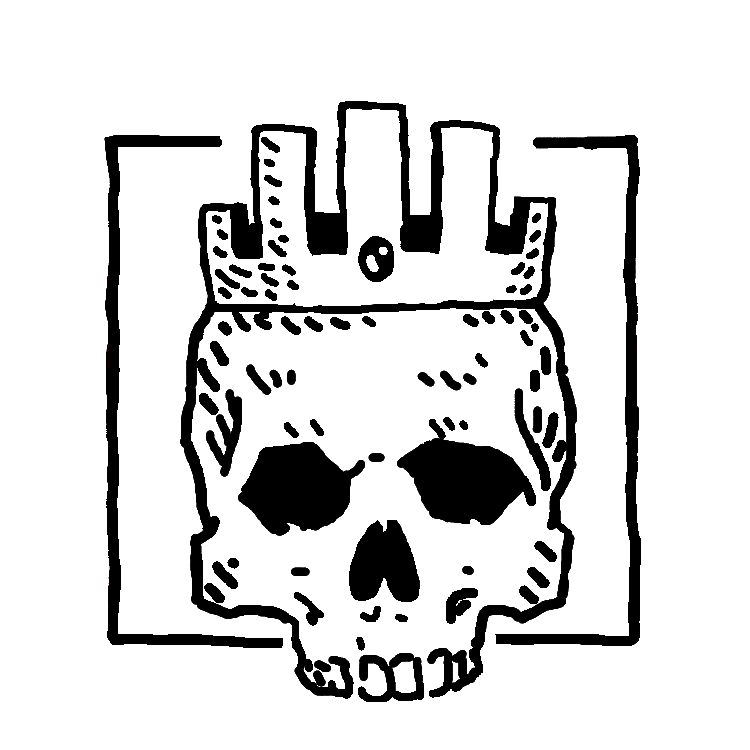
\includegraphics[width=\textwidth]{../Layout/pics/logo_character.png}
\end{minipage}\hfill
\begin{minipage}[c]{0.80\textwidth}
\flufffont{Characters represent the leaders and exceptional individuals who, through their particular sets of skills, influence the course of battle using either brute force, tactical acumen, spell casting ability, or engineering knowledge. It is they who muster the army, and your force will always include at least one representative of this Army Category to serve as your army General.}
\end{minipage}

\subsubsection{Core}

\begin{itemize}
\item This Army Category always has a minimum amount of points that must be spent on it, usually \SI{25}{\percent} of the Army Points.
\end{itemize}

\begin{minipage}[c]{0.17\textwidth}
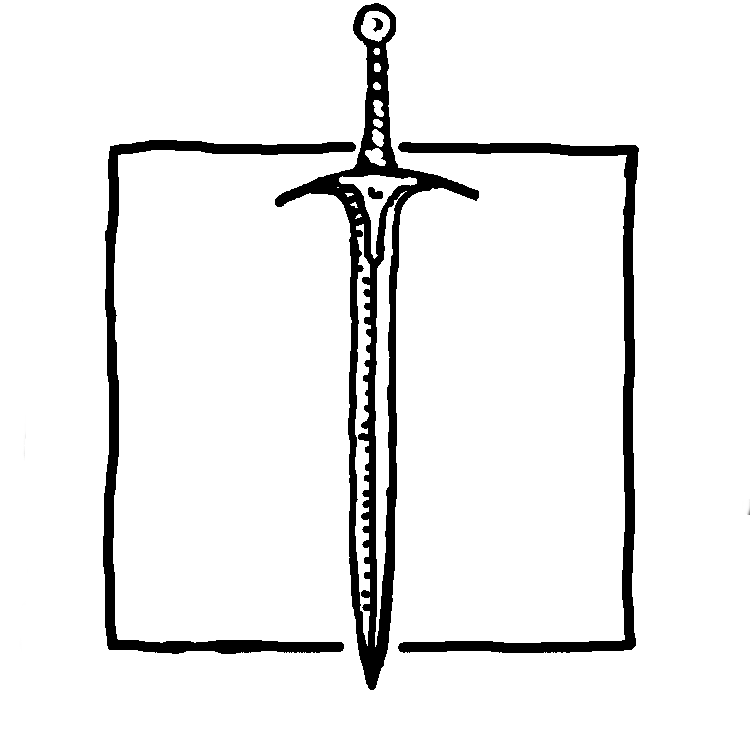
\includegraphics[width=\textwidth]{../Layout/pics/logo_core.png}
\end{minipage}\hfill
\begin{minipage}[c]{0.80\textwidth}
\flufffont{The Core represents the most readily available warriors a faction has access to and will form the bulk of combatants under the command of the Characters in the force. No matter where or why the faction fights, the Core are those units that will always be present in some combination as part of the fighting force. They are also those warriors that a society can provide for battle in the greatest numbers. While armies can overwhelmingly be formed out of the Core units, it is rarely the case as each commander seeks to deploy a force that contains as many of their finest or more specialised warriors as possible, depending on the resources available to them.}
\end{minipage}

\subsubsection{Special}

\begin{itemize}
\item This Army Category has no maximum or minimum limit. You are free to spend any amount of points on units in this Army Category, so long as the requirements of the army composition are met.
\end{itemize}

\begin{minipage}[c]{0.17\textwidth}
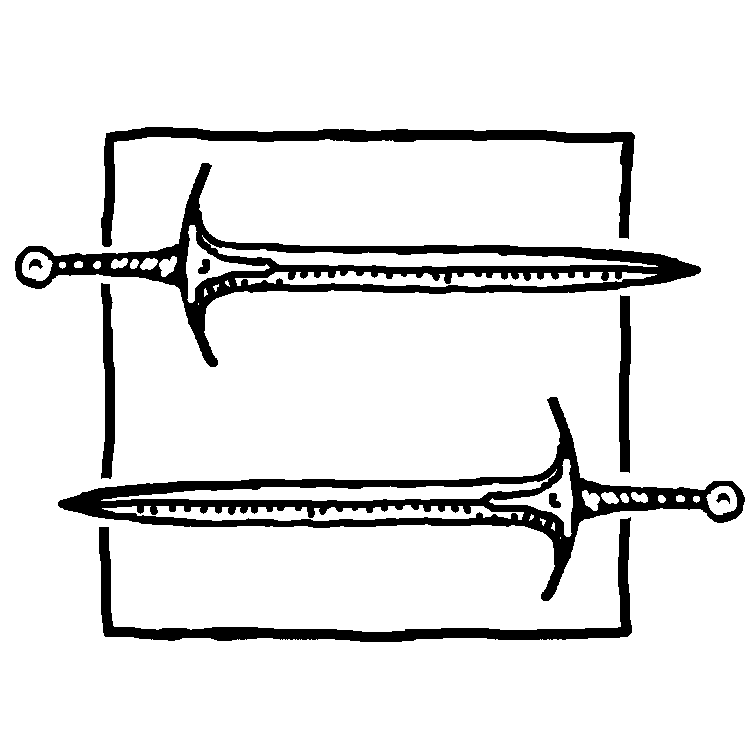
\includegraphics[width=\textwidth]{../Layout/pics/logo_special.png}
\end{minipage}\hfill
\begin{minipage}[c]{0.80\textwidth}
\flufffont{The Special Army Category represents more specialised warriors. A faction can call upon large numbers of these warriors and they can often be the most numerous segment of the entire fighting force. However, their numbers are still limited, and though some of these units can form an entire battle line there just isn't enough of them to form armies on their own.}
\end{minipage}

\subsubsection{Army-Specific}

\begin{itemize}
\item This Army Category has a maximum amount of points that can be spent on it; the limit is defined within individual Army Books.
\item All armies have one or more Army-Specific Categories.
\end{itemize}

\begin{minipage}[c]{0.17\textwidth}

\includegraphics[width=\textwidth]{../Layout/pics/logo_specific.png}
\end{minipage}\hfill
\begin{minipage}[c]{0.80\textwidth}
\flufffont{The Army-Specific Categories are introduced to provide additional limitations in the process of army building. These limitations are designed to be reflective of the nature of the faction in question, and with the goal of ensuring greater balance of the game. There are three types of Army-Specific Categories: one type is simply an additional grouping of units connected with a certain theme. These are given a thematic name reflective of the army they are part of or the function they perform (e.g. Orcs and Goblins -- Death from Above). The second type of Army-Specific Categories provides limitations linked with a certain function a unit from another Army Category performs within the army (e.g. Beast Herds -- Ambushers). And the third type of Army-Specific Categories is a mix of the above.}
\end{minipage}

\newpage
\subsubsection{Units Belonging to more than one Army Category}

Some units can be included in more than one Army Category, which is represented by more than one icon in their entry. In these cases, simply count the unit's Point Cost towards the limits of all its Army Categories, but only once towards the army Point Cost.

\subsubsection{Adding Army Categories}

Choosing certain options can make a unit count towards another Army Category in addition to its original Army Category. For example, giving a unit Shooting Weapons might make it also count towards the Ranged Support Army Category. This is marked by a small icon of the additional Army Category, displayed underneath the original Army Category icon(s), together with the conditions for counting in this additional Army Category.

\subsubsection{Splitting Point Cost between Army Categories}

In some rare cases a unit's Point Cost can be split between different Army Categories, where the Point Cost for some particular option is additionally counted towards a different Army Category than the unit. This is marked in the unit entry by a split icon, with the two halves representing the two Army Categories the unit counts towards.

For example, a 250 pts Elf Character, counted towards the Characters Army Category, decides to ride a 500 pts Dragon, which is an option marked to count additionally towards Beasts and Monsters. In this case, the player must count the entire unit's Point Cost (250 + 500 = 750 pts) towards Characters, and the Dragon's Point Cost (500 pts) towards Beasts and Monsters.

\subsection{Duplication Limits and Restrictions}
\idx[main=y]{Duplication Limits}\label{duplication_limits}

Certain units and options are limited in number in the army.

\subsubsection{0--X Items per Army}

Some items in the Army Books are marked with 0--X items per Army (e.g. 0--2 Units per Army, 0--2 Models per Army, 0--2 Mounts per Army). Such items can be included from zero to X times in the same army. The maximum limit (X) is halved for Warbands and doubled for Grand Armies, rounding fractions up (see below).

\subsubsection{\oneofakind}
\idx[main=y]{One of a Kind}

Items (units, upgrades, equipment, etc.) marked as \oneofakind{} may only be taken once per army. This is not changed for Warbands or Grand Armies.

\subsubsection{Minimum Army Size}
\idx[main=y]{Minimum Army Size}

Every army must contain a minimum of 4 units. Characters do not count towards this minimum. All units with the \hyperref[war_machine]{War Machine} Universal Rule together count as a single unit for this purpose.

\subsubsection{The General}
\idx[main=y]{General}\label{the_general}

A single Character in the army must be named the General. At least one Character must be included in the army that is eligible to fulfill this role. Who is the General must be noted on the Army List.

The General gains the \hyperref[commanding_presence]{\commandingpresence} Universal Rule.

\newpage
\section{Warbands and Grand Armies}
\idx[main=y]{Warbands}\idx[main=y]{Grand Armies}\label{warbands_and_grand_armies}

The rules for army composition are modified depending on the size of an army. An army that is unusually small or unusually large is subject to the following rules.

\begin{minipage}{0.5\textwidth -5pt}\begin{center}\textbf{Warbands}\end{center}\end{minipage}%
\hspace*{10pt}%
\begin{minipage}{0.5\textwidth -5pt}\begin{center}\textbf{Grand Armies}\end{center}\end{minipage}\vspace*{5pt}\newline%
\begin{tabular}{@{}p{0.5\textwidth -10pt}@{}p{20pt}@{}p{0.5\textwidth -10pt}@{}}
Armies of 3000 points or less are called Warbands. The Minimum Army Size is decreased to 3 units.&&%
Armies of 8000 points or more are called Grand Armies.\tabularnewline
All \enquote{0--X Items per Army} limits are halved, rounding fractions up.&&%
All \enquote{0--X Items per Army} limits are doubled.\tabularnewline
The usual board size is \distance{36} wide and \distance{48} deep.&&%
Adapt the board size to the size of the game.\tabularnewline
\end{tabular}

\section{How to Read Unit Entries}
\idx[main=y]{Unit Entries}\label{how_to_read_unit_entries}

Every unit in the game has a certain set of Characteristics and possibly optional or mandatory upgrades, and, as explained above, every unit is part of an Army Category. In addition, the models in that unit may be equipped with particular weapons and armour, and they may have one or more Model Rules, as you will learn in later chapters of this Rulebook (see \totalref{model_rules}).

Every unit is represented by its unit entry in its Army Book, and these unit entries contain all the information pertaining to that unit, including the data above as well as further information like Model Type and Height, base size, restrictions regarding the number of models or certain equipment, and so on.

This section will explain how the most common information in unit entries is presented in the Army Books of T9A.

\subsection{Common Unit Entries}

Unit entries usually consist of a header, the unit profile, and options, as illustrated in figure \ref{figure/common_unit_entry}.

\newcommand{\tinmen}{Tin Men}
\newcommand{\tinman}{Tin Man}
\newcommand{\tinmansheart}{Tin Man's Heart}
\newcommand{\tinmansheartdef}{The model must reroll failed to-hit rolls against every enemy models with Fear.}
\newcommand{\figTINMENHeader}{Header}
\newcommand{\figTINMENUnitProfile}{Unit\\ Profile}
\newcommand{\figTINMENOptions}{Options}

\begin{figure}[H]
	
\hspace*{0.12\textwidth}%
\begin{tikzpicture}[overlay]
	\draw [red,decorate,thick,decoration={brace,amplitude=6pt,mirror}]
(0,-0.18) -- (0.0,-1.4) node [black,midway,xshift=-0.9cm] 
{\figTINMENHeader};
	\draw [red,decorate,thick,decoration={brace,amplitude=6pt,mirror}]
(0.0,-1.47) -- (0.0,-4.25) node [align=right,black,midway,xshift=-0.9cm] 
{\figTINMENUnitProfile};
	\draw [red,decorate,thick,decoration={brace,amplitude=6pt,mirror}]
(0.0,-4.5) -- (0.0,-7.6) node [black,midway,xshift=-0.9cm] 
{\figTINMENOptions};
\end{tikzpicture}
\scalebox{0.8}{%
	\unitentry{%
		name=\tinmen{},
		logo=core,
		cost=120,
		unitsize=15,
		maxunitsize=50,
		costpermodel=10,
		maxunitsperarmy=4,
		scoring=yes,
		size=\sizestandard{},
		type=\infantry{},
		basesize=25\timess{}25,
		global@Ad=5,
		global@Ma=10,
		global@Di=7,
		globalrules={\scoring{},\strider{} (\forest{})},
		defense@HP=1,
		defense@Df=4,
		defense@Re=4,
		defense@Arm=2,
		defensearmour={\la{}},
		offensename=\tinman{},
		offense@At=1,
		offense@Of=4,
		offense@St=3,
		offense@AP=0,
		offense@Ag=3,
		offenserules={\textbf{\tinmansheart}},
		offenseweapons={\halberd{}},
		commandgroup={%
			\champion{}=20,
			\musician{}=20,
			\standardbearer{}=20,
			\alphaorderstickto{\standardbearer{}=20}\suboptionindent{}\bannerallowance{}=\nolimit{},
		},
		options={%
			\ambush{} ({\zerotoXmodelsperunit{25}, \zerotoXunitsperarmy{2}})=20,
			\onechoiceonlyACO{%
				\shield{}=1\permodel{},
				\pw{}=2\permodel{},
			},
			\throwingweapons{} (5+)=2\permodel{},
		},
		modelrulesdef={%
			\modelruledef{\tinmansheart}{\ruletype{\attackattributeclosecombat}\tinmansheartdef}
		},
		toggles={\togglefalse{twocolprintmodelrulesdef}\toggletrue{onecolprintmodelrulesdef}},
	} % END UNIT ENTRY
}

	\caption{Common unit entry.}
	\label{figure/common_unit_entry}
\end{figure}

\newpage
\subsubsection{Header}

The header of a unit entry usually contains all the general information on the unit (see figure \ref{figure/unit_entry_header}).

\newcommand{\figTMHOne}{1 -- Unit name}
\newcommand{\figTMHTwo}{2 -- Army Category}
\newcommand{\figTMHThree}{3 -- Unit size}
\newcommand{\figTMHFour}{4 -- Unit cost}
\newcommand{\figTMHFive}{5 -- Scoring}
\newcommand{\figTMHSix}{6 -- Unit cap}
\newcommand{\figTMHSeven}{7 -- Model specifications}

\begin{figure}[H]
		
\centering
\vspace*{0.8cm}%
\begingroup
	% Scaling down fonts by a 0.8 factor
	\normalfontsize%
	\renewcommand{\ChLab}[1]{{\fontsize{6.4}{7.68}\selectfont\greytextcolor{\textit{#1}}}} % Font for Characteristic's labels
	\renewcommand{\largerfontsize}{\fontsize{9.6}{11.52}\selectfont}%
	\renewcommand{\Largerfontsize}{\fontsize{12}{14.4}\selectfont}%
	\def\@minipagerestore{\setlength{\parskip}{\mycurrentparskip}}%
	\setlength{\lengthbeforemodelsize}{5.2cm}
	\begin{minipage}{0.8\textwidth}%
	\rule{\textwidth}{0.4pt}\par\vspace{-4pt}%
	% Logos
	\hspace*{-2.4pt}%
	\begin{minipage}[b]{0.08\textwidth}%
	\strut\tikz[remember picture] \node [inner sep=0pt] (ArmyCategory) {\includegraphics[width=\textwidth]{{logo_core}.png}};\strut%
	\vspace*{-3.2pt}%
	\end{minipage}%
	%
	% Title, unit cost and size
	\setlength{\lengthbeforemodelsizetwologos}{\lengthbeforemodelsize - 0.08\textwidth}
	\hspace{0.01\textwidth}\begin{minipage}[b]{0.5\textwidth+3pt}%
	% Title with hyperlink, scoring logo
	\strut\tikz[remember picture] \node [inner sep=0pt] (UnitName) {\Largerfontsize\textbf{\tinmen}};\strut%
	\vspace*{3pt}\newline%
	% Unit cost and size
	\strut\tikz[remember picture] \node [inner sep=0pt] (UnitCost) {\strut{\largerfontsize\pts{\textbf{120}}} + \pts{\textbf{10}}\perextramodel{}\strut};\strut%
	\hspace*{\lengthbeforemodelsize}%
	\setlength{\lengthoftheptsblock}{\widthof{{\largerfontsize\pts{\textbf{120}}} + \pts{\textbf{10}}\perextramodel{}}}%		
	\hspace*{-\lengthoftheptsblock}\hspace*{-1.5pt}%
	\strut\tikz[remember picture] \node [inner sep=0pt] (UnitSize) {\strut\textbf{15--50} \Models{}\strut};\strut%
	\vspace{0pt}%
	\end{minipage}%
	%
	% Restrictions
	\hfill\begin{minipage}[b]{0.2\textwidth}%
	\setlength{\parskip}{0pt}%
	\begin{center}%
		\strut\tikz[remember picture] \node [inner sep=0pt] (Scoring) {
\includegraphics[height=9.6pt]{logo_scoring.png}};\strut\par%
		\strut\tikz[remember picture] \node [inner sep=0pt] (UnitCap) {\strut\zerotoXunitsperarmy{4}};\strut\par%
	\end{center}%
	\vspace{0pt}%
	\end{minipage}%
	%
	% Size, Type and Base
	\begin{minipage}[b]{0.2\textwidth}%
	\renewcommand{\arraystretch}{1}%
	\strut\tikz[remember picture] \node [inner sep=0pt] (ModelSpecifications) {%
		\begin{tabular}{@{}>{\raggedleft}p{0.25\textwidth}@{\hskip 0.03\textwidth}p{0.72\textwidth}@{}}%
		\ChLab{\size}&\sizestandard{}\tabularnewline%
		\ChLab{\type}&\infantry{}\tabularnewline%
		\ChLab{\basesize}&25\timess{}25 \si{\milli\meter}%
		\tabularnewline%
		\end{tabular}%
	};\strut%
	\vspace*{-3.2pt}%
	\end{minipage}\vspace{-2pt}\par%
	\vspace{-10pt}\rule{\textwidth}{0.4pt}\par%
	\end{minipage}
\endgroup
\vspace*{0.8cm}%
\newlength{\unitnameboxwidth}%
\setlength{\unitnameboxwidth}{\widthof{\Largerfontsize\textbf{\tinmen}}}%
\newlength{\unitnameboxheight}%
\setlength{\unitnameboxheight}{\heightof{\Largerfontsize\textbf{\tinmen}}}%
\newlength{\armycategoryboxwidth}%
\setlength{\armycategoryboxwidth}{0.064\textwidth}%
\newlength{\armycategoryboxheight}%
\setlength{\armycategoryboxheight}{\heightof{\includegraphics[width=0.064\textwidth]{{logo_core}.png}}}%
\newlength{\unitcostboxwidth}%
\setlength{\unitcostboxwidth}{\widthof{{\largerfontsize\pts{\textbf{120}}} + \pts{\textbf{10}}\perextramodel{}}}%
\newlength{\unitcostboxheight}%
\setlength{\unitcostboxheight}{\heightof{{\largerfontsize\pts{\textbf{120}}} + \pts{\textbf{10}}\perextramodel{}}}%
\newlength{\unitsizeboxwidth}%
\setlength{\unitsizeboxwidth}{\widthof{\textbf{15--50} \Models{}}}%
\newlength{\unitsizeboxheight}%
\setlength{\unitsizeboxheight}{\heightof{\textbf{15--50} \Models{}}}%
\newlength{\unitcapboxwidth}%
\setlength{\unitcapboxwidth}{\widthof{\zerotoXunitsperarmy{4}}}%
\newlength{\unitcapboxheight}%
\setlength{\unitcapboxheight}{\heightof{\zerotoXunitsperarmy{4}}}%
\newlength{\scoringboxwidth}%
\setlength{\scoringboxwidth}{\widthof{
\includegraphics[height=9.6pt]{logo_scoring.png}}}%
\newlength{\scoringboxheight}%
\setlength{\scoringboxheight}{9.6pt}%
\begin{tikzpicture}[remember  picture, overlay, highlight/.style = {draw=red,rounded corners=3pt,thick},comment/.style = {align=center, fill= black!5,minimum height=0.55cm},every edge/.append style = { ->, thick, >=stealth,black!50,dashed,line width=1pt},]
	\node [highlight,minimum width=\unitnameboxwidth-2pt,minimum height=\unitnameboxheight+2pt] (UnitNameFrame) at (UnitName) {};
	\node [highlight,minimum width=\armycategoryboxwidth-2pt,minimum height=\armycategoryboxheight+2pt] (ArmyCategoryFrame) at (ArmyCategory) {};
	\node [highlight,yshift=0.05cm,minimum width=\unitcostboxwidth-18pt,minimum height=\unitcostboxheight+3pt] (UnitCostFrame) at (UnitCost) {};
	\node [highlight,yshift=0.03cm,minimum width=\unitsizeboxwidth-4pt,minimum height=\unitsizeboxheight+3pt] (UnitSizeFrame) at (UnitSize) {};
	\node [highlight,yshift=0.02cm,minimum width=\unitcapboxwidth-8pt,minimum height=\unitcapboxheight+3pt] (UnitCapFrame) at (UnitCap) {};
	\node [highlight,minimum width=\scoringboxwidth+8pt,minimum height=\scoringboxheight+4pt,yshift=1pt] (ScoringFrame) at (Scoring) {};
	\node [highlight,minimum width=2.6cm,minimum height=1.1cm,xshift=-0.3cm,yshift=0.035cm] (ModelSpecificationsFrame) at (ModelSpecifications) {};
	\node [comment,above right= 1cm and 0.4cm of ArmyCategoryFrame.center] (UnitNameComment) {\figTMHOne};
	\node [comment,right=1.8cm of UnitNameComment] (UnitSizeComment) {\figTMHThree};
	\node [comment,right=1cm of UnitSizeComment] (ScoringComment) {\figTMHFive};
	\node [comment,right=1cm of ScoringComment] (ModelSpecificationsComment) {\figTMHSeven};
	\node [comment,below= 1cm of ArmyCategoryFrame.center] (ArmyCategoryComment) {\figTMHTwo};
	\node [comment,right=1cm of ArmyCategoryComment] (UnitCostComment) {\figTMHFour};
	\node [comment,right=3.3cm of UnitCostComment] (UnitCapComment) {\figTMHSix};
	\draw (UnitNameComment) edge (UnitNameFrame);
	\draw (UnitSizeComment) edge (UnitSizeFrame);
	\draw (ScoringComment) edge (ScoringFrame);
	\draw (ArmyCategoryComment) edge (ArmyCategoryFrame);
	\draw (UnitCostComment) edge (UnitCostFrame);
	\draw (UnitCapComment) edge (UnitCapFrame);
	\draw (ModelSpecificationsComment) edge (ModelSpecificationsFrame);
\end{tikzpicture}
	
	% If the translated output doesn't look right, we'll need to design a unit_entry_header.tex specific for each language, please contact Eru.
	\caption{Header of a common unit entry.}
	\label{figure/unit_entry_header}
\end{figure}

\paragraph{1 -- Unit name}

This is the name of the unit that will be used e.g. when choosing the unit to perform an action like Charging, or when targeting the unit with a spell or a Shooting Attack.

\paragraph{2 -- Army Category}

Every unit is part of an Army Category, like Characters, Core, or Special, which is important e.g. for building an army or for certain Model Rules. Each Army Category is represented by an icon that corresponds to the respective Army Category as shown in each Army Book's section on Army Organisation.

Note that some units may belong to more than one Army Category (see \totalref{army_categories}). In this case the icons of all these Army Categories will be depicted.

\paragraph{3 -- Unit size}

The unit size tells you the minimum and the maximum size of the unit when building an army. The minimum unit size corresponds to the number of models that the unit must contain at least. And accordingly, the maximum unit size represents the number of models that the unit can consist of at the most.

In the example in figure \ref{figure/unit_entry_header}, a unit of Tin Men must consist of at least 15 models when building the army, while you can add up to 35 models, attaining the unit's maximum size of 50 models.

\paragraph{4 -- Unit cost}

The unit cost tells you how many points you have to pay for adding the unit to your army in its minimum size, and how many points each additional model will cost. For some units in the game, an additional model will cost the same amount of points as a model that is part of the unit's minimum size, while for others additional models may be more or less expensive than the initial models.

In the example in figure \ref{figure/unit_entry_header}, a unit of Tin Men consisting of the minimum size of 15 models will cost 120 points, while each additional Tin Man model will cost 10 points. So for instance a unit of 25 Tin Men will cost a total of 220 points (120 points for the first 15 models and 100 pts for the 10 additional models).

\paragraph{5 -- Scoring}

Some units have a certain Model Rule called Scoring, which is relevant for winning Secondary Objectives during the game (see \totalref{scoring} and \totalref{secondary_objectives}). Units with this Model Rule will be marked with a pennant icon.

\paragraph{6 -- Unit cap}

Certain units can only be selected a limited number of times in an army. In this case you will find a \enquote{\zerotoXunitsperarmy{X}} cap in the unit entry. In the example, an army may contain up to two units Tin Men, regardless of their size, equipment, etc.

\paragraph{7 -- Model specifications}

Every model in the game has a specific Height, Type, and base size, which are relevant for a wide variety of game mechanics and Model Rules.

\subsubsection{Unit Profile}

The unit profile contains the models' Characteristic Profiles and Model Rules, including their mundane equipment (see figure \ref{figure/unit_profile}).

\newcommand{\tinmenglobalrules}{\scoring{},\strider{} (\forest{})}
\newcommand{\tinmendefrules}{\la}
\newcommand{\tinmenoffrules}{\textbf{\tinmansheart}}
\newcommand{\tinmenoffweapons}{\halberd}

\newcommand{\figTINMENProfileEight}{8 -- Characteristic Profiles}
\newcommand{\figTINMENProfileNine}{9 -- Model Rules}

\begin{figure}[H]
	\centering
	
\vspace*{0.6cm}
\begin{tikzpicture}[overlay]
	\draw [red,decorate,thick,decoration={brace,amplitude=6pt}]	(0.1,1.58) -- (6.88,1.58) node [black,midway,align=center,yshift=0.45cm] {\figTINMENProfileEight};
	\draw [red,decorate,thick,decoration={brace,amplitude=6pt}]	(6.95,1.58) -- (13.65,1.58) node [black,midway,align=center,yshift=0.45cm] {\figTINMENProfileNine};
\end{tikzpicture}
\scalebox{0.8}{%
	\def\@minipagerestore{\setlength{\parskip}{\mycurrentparskip}}%
	\hbadness=10000%
	\begin{minipage}{\textwidth}
		%%%%%%%%%%%%%%%%%%%%%%
		% Characteristics and rules
		%%%%%%%%%%%%%%%%%%%%%%
		% Global Characteristics
		\renewcommand{\arraystretch}{1.4}%
		\startcharacteristicstable{}%
			\hspace*{3pt}{\ChLab{\GlobalCharacteristics}}&%
			{\ChLab{\AdvanceRateInitials}}&%
			{\ChLab{\MarchRateInitials}}&%
			{\ChLab{\DisciplineInitials}}&%
			&%
			&%
			\ChLab{\ModelRules}\tabularnewline%
			&%
			\ChVal{\distance{5}}%
			&%
			\ChVal{\distance{10}}%
			&%
			\ChVal{7}&%
			&%
			&%
			\strut\alphaorderlist{\tinmenglobalrules}%
			\tabularnewline%
		\end{tabular}%
		
		%%%%%%%%%%%%%%%%%%%%%%
		% Defensive Characteristics
		\vspace*{-7pt}%
		\startcharacteristicstable{}%
			\hspace*{3pt}\ChLab{\DefensiveCharacteristics{}}&%
			{\ChLab{\HealthPointsInitials}}&%
			{\ChLab{\DefensiveSkillInitials}}&%
			{\ChLab{\ResilienceInitials}}& %
			{\ChLab{\ArmourInitials}}&%
			&%
			\tabularnewline%
			&% no defensive name
			\ChVal{1}&%
			\ChVal{4}&%
			\ChVal{4}&%
			\ChVal{2}&%
			&%
			\strut\alphaorderlist{\tinmendefrules}%
			\tabularnewline%
		\end{tabular}%
		
		%%%%%%%%%%%%%%%%%%%%%%
		% Offensive Characteristics
		\vspace*{-7pt}%
		\startcharacteristicstable{}%
			\hspace*{3pt}\ChLab{\OffensiveCharacteristics{}}&%
			{\ChLab{\AttackValueInitials}}&%
			{\ChLab{\OffensiveSkillInitials}}&%
			{\ChLab{\StrengthInitials}}& %
			{\ChLab{\ArmourPenetrationInitials}}&%
			{\ChLab{\AgilityInitials}}&%
			\tabularnewline%
			&%
			\ChVal{1}&%
			\ChVal{4}&%
			\ChVal{3}&%
			\ChVal{0}&%
			\ChVal{3}&%
			\strut\alphaorderlist{\tinmenoffrules}%
			, %
			\alphaorderlist{\tinmenoffweapons}%
			\tabularnewline%
		\end{tabular}\newline%
	\end{minipage}
}

	\caption{Unit profile of a common unit entry.}
	\label{figure/unit_profile}
\end{figure}

\paragraph{8 -- Characteristic Profiles}

The Characteristic Profiles of each unit entry contain the values of all of a unit's Global, Defensive, and Offensive Characteristics. Note that the values displayed here represent the models' unmodified Characteristic values, excluding any modifiers e.g. from Model Rules and equipment:

\begin{itemize}
\item For instance, in case of Armour, the Characteristic value displayed here represents the models' innate armour (granted e.g. from scales or a tough hide). Any armour from Armour Equipment, like Light Armour in the example above, will have to be added on top of the Armour value displayed in the Defensive Profile. In this example, the models will have an Armour of 3 (2 from the models' innate armour and 1 from their Light Armour), which will give them a 4+ Armour Save against attacks without any Armour Penetration (see \totalref{armour_saves}).
\item The profile also displays the models' unmodified Strength and Armour Penetration. Any Strength and Armour Penetration modifiers, e.g. from weapons, will have to be added on top. In our example, the models' Close Combat Attacks will have a Strength value of 4 and an Armour Penetration value of 1, due to the innate Strength of 3 and the +1 Strength and Armour Penetration modifiers from the Halberds the models are equipped with.
\end{itemize}

\paragraph{9 -- Model Rules}

In this part of the unit entry, the unit's Model Rules are displayed:

\begin{itemize}
\item The Global Model Rules comprise the unit's Universal Rules (in alphabetical order).
\item The Defensive Model Rules comprise the unit's Personal Protections and Armour Equipment. In case a unit has more than one Model Rule from these categories, Personal Protections will be listed first (in alphabetical order), followed by the unit's Armour Equipment (in alphabetical order).
\item The Offensive Model Rules comprise the unit's Attack Attributes, Special Attacks, and weapons. In case a unit has more than one Model Rule from these categories, Attack Attributes and Special Attacks will be listed first (in alphabetical order), followed by the unit's weapons (in alphabetical order).
\end{itemize}

In some unit entries, you will notice certain Model Rules in bold, like Tin Man's Heart in the example above. Bold font is used here to highlight army-specific Model Rules that are defined in the unit entry.

\newpage
\subsubsection{Options}

In this part of the unit profile illustrated in figure \ref{figure/unit_entry_options}, you will find all the optional and mandatory upgrades that can be bought for a unit when building the army.

\newcommand{\figTINMENOptionsTen}{10 -- Command Group Options}
\newcommand{\figTINMENOptionsEleven}{11 -- Unrestricted\\ options}
\newcommand{\figTINMENOptionsTwelve}{12 -- Restricted\\ options}
\newcommand{\figTINMENOptionsThirteen}{13 -- Model Rules}

\begin{figure}[H]
	
\newcommand{\TINMENoptions}{%
	\ambush{} ({\zerotoXmodelsperunit{25}, \zerotoXunitsperarmy{2}})=20,
	\onechoiceonlyACO{%
		\shield{}=1\permodel{},
		\pw{}=2\permodel{},
	},
	\throwingweapons{} (5+)=2\permodel{},	
}
\newcommand{\TINMENcommandgroup}{%
	\champion{}=20,
	\musician{}=20,
	\standardbearer{}=20,
	\alphaorderstickto{\standardbearer{}=20}\suboptionindent{}\bannerallowance{}=\nolimit{},	
}
\newcommand{\TINMENmodelrules}{%
	\modelruledef{\tinmansheart}{\ruletype{\attackattributeclosecombat}\tinmansheartdef}
}	
\vspace*{0.3cm}
\hspace*{0.18\textwidth}%
\begin{tikzpicture}[overlay]
	\draw [red,decorate,thick,decoration={brace,amplitude=6pt}]	(6.95,1.63) -- (13.7,1.63) node [black,midway,align=center,yshift=0.45cm] {\figTINMENOptionsTen};
	\draw [red,decorate,thick,decoration={brace,amplitude=6pt,mirror}]
(0.0,1.58) -- (0.0,0.03) node [align=right,black,midway,left=0.2cm] 
{\figTINMENOptionsTwelve};
	\draw [red,decorate,thick,decoration={brace,amplitude=2.5pt,mirror}]
(0.0,-0.02) -- (0.0,-0.5) node [align=right,midway,black,left=0.2cm] 
{\figTINMENOptionsEleven};
%	\draw [->,red,thick]
%(0.1,-0.2) -- (-0.2,-0.2) node [align=right,black,left=0cm] 
%{\figTINMENOptionsEleven};
	\draw [red,decorate,thick,decoration={brace,amplitude=6pt,mirror}]
(0.0,-0.55) -- (0.0,-1.6) node [align=right,black,midway,left=0.2cm] 
{\figTINMENOptionsThirteen};
\end{tikzpicture}
\scalebox{0.8}{%
	\def\@minipagerestore{\setlength{\parskip}{\mycurrentparskip}}%
	\hbadness=10000%
	\begin{minipage}{\textwidth}
		\setlength{\columnsep}{10pt}%
		\setlength{\multicolsep}{0pt}%
		\raggedcolumns%
		\begin{multicols}{2}%
			\strut\options{\TINMENoptions}%
			\strut\commandgroup{\TINMENcommandgroup}%
		\end{multicols}%
		% Additional space if there is a single column rule after
		\vspace*{8pt}%
		% Single column
		\vspace*{-5pt}%
		\strut\modelrulesdef{\TINMENmodelrules}%
	\end{minipage}
}

	\caption{Options in a common unit entry.}
	\label{figure/unit_entry_options}
\end{figure}

\paragraph{10 -- Command Group options}

Certain units have one or more Command Group Options in their unit entry, which allow them to upgrade one model of the unit to a Champion, another model to a Musician, and another model to a Standard Bearer. This means that a single \rnf{} model cannot be upgraded to be a Musician and a Standard Bearer at the same time. In addition, each unit can only upgrade models to a single Champion, a single Musician, and a single Standard Bearer.

Note that upgrading the unit with a Champion/Musician/Standard Bearer does not grant you extra models for the unit as you upgrade models that are already part of the unit.

Some Command Group models have additional options for upgrades, for instance the Standard Bearer in the example above can purchase a Banner Enchantment. These options are listed indented underneath the corresponding Command Group model. In order to have access to such an additional upgrade, you must first upgrade a model to the corresponding Command Group model, and only then you can buy the upgrade for that model.

\paragraph{11 -- Unrestricted options}

Many units have options to upgrade their models with weapons, armour, certain Model Rules, etc. In some cases, the Point Cost per unit is indicated, regardless of the number of models, while in others, like in the example above, the unit entry gives the Point Cost per model.

Note that if you choose to buy such an upgrade, you must always upgrade all models of the unit accordingly.

\paragraph{12 -- Restricted options}

Certain options may come with restrictions. These may for instance be associated with an altered maximum number of models per unit (in the example above 25 instead of 50), or with a restriction regarding the number of units with the upgrade an army may contain (up to 2 units in the example above). Another possible restriction is an upper limit on the total number of models with a given upgrade per army. In this case, the sum of all models of all units with that upgrade in the army may not exceed that upper limit.

Other options cannot be combined with one another. These are listed indented underneath \enquote{One choice only} in the unit entry. In the example above, the models in the unit may be upgraded either with Shields or with Paired Weapons, they may however not gain Shields and Paired Weapons.

In case there are several groups of these \enquote{One choice only} upgrades for a unit, the unit may be given up to one choice of each group.

\paragraph{13 -- Model Rules}

In case a unit profile contains any unit-specific Model Rules, these rules will be explained in this part of the unit entry.

\subsection{Complex Unit Entries}

In addition to the elements detailed above, certain units may have additional distinctive features that will be explained based on the Character unit entry in figure \ref{figure/complex_unit_entry}.

\newcommand{\wickedwitch}{Wicked Witch}
\newcommand{\hydrophobe}{Hydrophobe}
\newcommand{\hydrophobedef}{%
If the model touches a Water Terrain Feature, it is immediately removed as a casualty.%
}
\newcommand{\redrubberboots}{Red Rubber Boots}
\newcommand{\redrubberbootsdef}{%
The model loses the \hydrophobe{} Model Rule and gains \strider{} (Water Terrain).%
}
\newcommand{\witchesbroom}{Witches' Broom}
\newcommand{\wingedmonkeychariot}{Winged Monkey Chariot}

\begin{figure}[H]
	\centering
	
\begin{tikzpicture}[overlay,every node/.style={draw=red,circle,thick, inner sep=0pt,minimum size=12pt}]
	\node at (7.3,-0.65) {\textcolor{red}{a}};
	\node at (9.6,-0.65) {\textcolor{red}{b}};
	\node at (0.4,-6) {\textcolor{red}{c}};
	\node at (6.95,-5.15) {\textcolor{red}{d}};
	\node at (6.85,-6.5) {\textcolor{red}{e}};
	\node at (-0.25,-8.4) {\textcolor{red}{f}};
\end{tikzpicture}
\scalebox{0.8}{%
	\unitentry{%
		name=\wickedwitch{},
		logo=character,
		cost=140,
		unitsize=1,
		maxunitsperarmy=3,
		type=\infantry{},
		size=\sizestandard{},
		basesize=20\timess{}20,
		global@Ad=5,
		global@Ma=10,
		global@Di=8,
		globalrules={\textbf{\hydrophobe},\wizardapprentice{}},
		defense@HP=3,
		defense@Df=4,
		defense@Re=3,
		defense@Arm=0,
		offensename=\wickedwitch{},
		offense@At=1,
		offense@Of=4,
		offense@St=3,
		offense@AP=0,
		offense@Ag=5,
		magic={\wizardadept{}=75,\wizardmaster{}=225,},
		paths={\cosmology{}=cosmology,\druidism{}=druidism,\witchcraft{}=witchcraft},
		options={%
			\specialequipmentallowance{}=\upto{}100,
			\suboptionindent\ifwizardmaster{}=\upto{}200,
			\textbf{\redrubberboots}=5,
		},
		mounts={%
			\witchesbroom{}=30,
			\wingedmonkeychariot{}=200,
		},
		modelrulesdef={%
			\modelruledef{\hydrophobe}{\ruletype{\universalrule}\hydrophobedef}%
		},
		optionalmodelrulesdef={%
			\modelruledef{\redrubberboots}{\ruletype{\universalrule}\redrubberbootsdef}%
		},
		toggles={%
			\toggletrue{onecolprintmodelrulesdef}\togglefalse{twocolprintmodelrulesdef}
			\toggletrue{onecolprintoptionalmodelrulesdef}\togglefalse{twocolprintoptionalmodelrulesdef}
		},
	}	
}

	\caption{Character unit entry.}
	\label{figure/complex_unit_entry}
\end{figure}

a) Certain units, like Characters, consist only of a single model. These units are labelled as \enquote{single model} units. They follow the same rules as units consisting of multiple models, but there may be certain differences, like Characters being able to join other units.

b) Just like regular units, Characters may have a unit cap. This cap applies to all Characters of this type, regardless of their upgrades, equipment, and mounts. In this example, this means that you can only have up to 3 Wicked Witches in your army, e.g. one of them on foot and two on Witches' Brooms.

c) Models that can cast spells are referred to as Wizards. Wizards come in 3 different types: Wizard Apprentice, Adept, and Master. The Model Rules tell you which Wizard type the model has by default (in this example, the Wicked Witch is a Wizard Apprentice), while the Magic Options show you which types the model can be upgraded to. In case you upgrade your Wizard, the upgrade replaces the default Wizard type. In addition, you will also find in this section the Paths that the Wizard has to choose a single one from. The Wizard will select its spells from this chosen Path (see \totalref{spell_selection}).

d) Certain models, like most Characters, have access to Weapon Enchantments, Armour Enchantments, Artefacts, etc. These upgrades are referred to as Special Items (see \totalref{special_items} and \nameofthegame{} -- Arcane Compendium). If a model can buy Special Items, you will find this information in the unit entry's options, together with the maximum amount of points a model can spend on them.

e) Characters are usually on foot by default. Most of them can however be given a mount. The Mount Options will tell you which mounts are available for a Character and how many points you have to pay for them. Note that a Character may always only take a single mount.

f) As explained above, unit entries will contain unit-specific Model Rules. In addition, you will sometimes also find Optional Model Rules. In order to gain these Model Rules, you must buy the corresponding upgrade for the model.

\newpage
\subsection{Unit Entries with Multipart Models}

The examples above show entries of units with models consisting of a single model part, but there are also many Multipart Models in the game (see \totalref{multipart_models}). The unit entry of a Character Mount, the Winged Monkey Chariot from the example in figure \ref{figure/unit_entry_multipart_model}, will be used to explain the particularities of this type of unit entry.

\newcommand{\crew}{Crew}
\newcommand{\wingedmonkey}{Winged Monkey}
\newcommand{\chassis}{Chassis}

\begin{figure}[H]
	\centering
	
\begin{tikzpicture}[overlay,every node/.style={draw=red,circle,thick, inner sep=0pt,minimum size=12pt}]
	\node at (9.6,-0.65) {\textcolor{red}{a}};
	\node at (5.6,-2.2) {\textcolor{red}{b}};
	\node at (-0.05,-4.7) {\textcolor{red}{c}};
\end{tikzpicture}
\scalebox{0.8}{%
	\unitentry{%
		name=\wingedmonkeychariot{},
		logo=character,
		maxmountsperarmy=1,
		type=\construct{},
		size=\sizelarge{},
		basesize=50\timess{}100,
		global@Ad=2,
		global@Ma=2,
		global@Adfly=9,
		global@Mafly=9,
		global@Di=\ascharacter{},
		globalrules={\fly{9}{9},\lighttroops{},\swiftstride{}},
		defense@HP=4,
		defense@Df=\ascharacter{},
		defense@Re=4,
		defense@Arm=\ascharacter{}+1,
		defenserules={\hardtarget{} (1)},
		offensename=\crew{} (2),
		offense@At=1,
		offense@Of=4,
		offense@St=3,
		offense@AP=0,
		offense@Ag=5,
		offenseweapons={\lightlance},
		offensenameB={\wingedmonkey{} (2)},
		offenseB@At=2,
		offenseB@Of=4,
		offenseB@St=4,
		offenseB@AP=1,
		offenseB@Ag=4,
		offenserulesB={\harnessed{},\hatred{}},
		offensenameI=\chassis{},
		offenseI@St=5,
		offenseI@AP=2,
		offenserulesI={\impacthits{D6},\inanimate{}},
	}
}

	\caption{Unit entry of a Multipart Model.}
	\label{figure/unit_entry_multipart_model}
\end{figure}

a) Like for any other unit entry, there may be restrictions on the number of Character Mounts that can be part of an army. In the example above, the army may only contain up to a single Character, regardless of the type, on a Winged Monkey Chariot. This restriction only applies to Character mounts, so if an Army Book contains the Character mount additionally as a unit in another Army Category, you are allowed to take this unit in addition to the Character mount in your army.

b) In case of a Multipart Model Character, many of a model's Characteristic values will be determined by the mount's Characteristics, unless they are marked with \enquote{C} or \enquote{C+X} in the mount's profile (see \totalref{special_cases_of_characteristic_values}), which refers to the value in the Character's profile. In this example, the mount does not have a proper Discipline Value, but the Multipart Model uses the Character's Discipline, which is 8.

c) Models consisting of a single model part have one Global, Defensive, and Offensive Profile each. Multipart Models also have one Global and Defensive Profile each, which apply to the entire Multipart Model. However, they do have a separate Offensive Profile for each identical model part. The mount above has 5 model parts: 2 Crew members and 2 Winged Monkey's (as indicated by the \enquote{2} in brackets) and a Chassis, which all have their own Offensive Profile.

\newpage
\section{Hidden and Open Lists}
\idx{Army Lists}\idx[main=y]{Open Lists}\idx[main=y]{Hidden Lists}\label{hidden_and_open_lists}

Rules are written and balanced based on the principle of openness, and we encourage players to share their full Army Lists with their opponents at the start of the game. This Army List should include all units, unit options, Special Items, special abilities, Point Costs, and so on. The only things that are not open to your opponent are things that are explicitly stated as hidden or secret.

\begin{optionalrules}
\subsection{Optional Rules for Hidden Lists}
\label{optional_rules_for_hidden_lists}

Some players may prefer to use so-called hidden lists, and for those players we have included the hidden list rules. Please note that the game is not balanced with these rules in mind. In this format, most of your Army List will be open, meaning that your opponent should know what your army consists of before the game starts. However, some parts of your army are secret or \enquote{hidden}. Both players should provide their opponent with the open part of their army before the game begins, referred to as a mundane Army List.

The following elements are included in the hidden part of your army:

\begin{itemize}
\item Special Items that are picked from the List of Common Special Items given in \nameofthegame{} -- Arcane Compendium
\item Special Items that are specific to Army Books, as well as any option that follows the rules for Special Items such as Daemonic Items and Dwarven Runic Items
\end{itemize}

Anything not on this list belongs to the mundane Army List.

If an army has two or more units or models that are identical regarding their open part but have hidden differences, the player must be able to tell the units apart in the hidden list. For example if a player fields two units identical in every way except that one has an enchanted banner and the other doesn't, the Army List may specify that the unit with the enchanted banner has a red banner while the unit with a blue banner possesses no such Special Item.

\subsubsection{Revealing Special Items}

Special Items (or similar) must be revealed the first time they are used. A Special Item is considered as being used when it affects or could affect the game in any way. For example:
\begin{itemize}
\item It affects a dice roll (even if the actual result of the dice has no effect).
\item It alters an attack (such as an enchanted weapon, or any Special Item with a rule that affects an attack).
\item It alters a saving roll (reveal the Special Item before making the saving roll). Note that a Special Item that affects the saving roll the same way as the non-Enchanted counterpart would does not need to be revealed.
\end{itemize}

A Special Item that increases movement only counts as being used if the unit moves farther than it could without it or when Charging (declare that you have the Special Item before rolling the Charge Range but after Charge Reactions are resolved).

When revealing Dwarven Runic Items, only reveal the Rune that is being used, not the entire combined item.
\end{optionalrules}\debugfooter % Else footer goes wild for some reason with ocgcolorlinks option
